\documentclass[a4paper,11pt]{report}

\usepackage[frenchb]{babel}
\usepackage[utf8]{inputenc}
\usepackage{wrapfig}
\usepackage{graphicx}
\usepackage {amsmath}
\usepackage{amssymb}
\usepackage{amsthm}
\usepackage{mathrsfs}
\usepackage{soul}
\usepackage{algorithm,algorithmic}
\usepackage{listings}
\usepackage[toc,page]{appendix} 
\usepackage{ulem}
\usepackage[top=2.5cm, bottom=3cm, left=3cm, right=3cm]{geometry}

\renewcommand{\thepage}{}

\begin{document}

%%%%%%%%%%%%%%%%%%%%%%%%%%%%%%%%%%%%%%%%%%%%%%%%%%%

\lstset {
	language=java,
	morekeywords={def, object, val, var, Int}
}
\begin{figure}
   
\includegraphics[scale = 0.75]{HeaderPagedeGarde.PNG}
\end{figure}
\author{Maxime Escourbiac - Jean-Christophe Septier \\ Responsable ISIMA : Jonathan PASSERAT-PALMBACH \& Romain REUILLON}
\title{
   Rapport de projet \\ 3ème année ingénieur \\Génération de code OpenCl\\
  \bigskip
}
\date{\today}
\maketitle

%%%%%%%%%%%%%%%%%%%%%%%%%%%%%%%%%%%%%%%%%%%%%%%%%%%
\newpage

\begin{flushleft}
\LARGE{ \bf {Remerciements:}\bigskip}
\end{flushleft}

\normalsize{

Nous tenons à remercier {\bf Jonathan PASSERAT-PALMBACH} , qui nous a épaulés pour la réalisation de ce projet. Il a été très présent pour nous apporter son aide et ses conseils.
\\ \\
Nous remercions {\bf Romain REUILLON} pour nous avoir aidés à débuter le projet lors de réunions.
\\ \\
Nous remercions également {\bf Olivier CHAFIK}, qui nous a apporté son aide lors du développement de notre solution, afin d’intégrer nos modifications à son projet. 

}

%%%%%%%%%%%%%%%%%%%%%%%%%%%%%%%%%%%%%%%%%%%%%%%%%%%%
\newpage
%table des figures et des illustrations

\listoffigures

%%%%%%%%%%%%%%%%%%%%%%%%%%%%%%%%%%%%%%%%%%%%%%%%%%%%
\newpage
\begin{flushleft}
\LARGE{ \bf {Résumé:}\bigskip}
\end{flushleft}

\normalsize{
Dans le domaine de la simulation, il est nécessaire de réaliser un certain nombre de réplications d'une même expérience, afin d'obtenir des résultats statistiquement corrects. Pour réduire le temps d'exécution de ces réplications, la parallélisation est utilisée. Un des moyens utilisés pour paralléliser est l'emploi de GPU (Graphics Processing Units). Cette solution permet à faible coût d'exécuter les mêmes opérations grâce aux threads : les nombreuses unités de calcul parallèle disponibles sur un GPU.\\

Les chercheurs du LIMOS ont proposé une publication proposant une nouvelle approche de parallélisation, permettant de résoudre une limitation matérielle des GPU au niveau de l'accès à la mémoire vive et des exécutions de codes indépendants. Cette solution se nomme Warp-Level-Parallelism.\\

Notre projet a consisté à implémenter ce paradigme dans un langage de haut niveau, nommé ScalaCL. ScalaCL est un projet Open Source créé par Olivier Chafik, permettant de générer du code OpenCL à partir d'un code Scala.\\

La première étape de notre projet a été d'analyser la publication afin de comprendre l'intérêt de ce nouveau paradigme pour la réplication de simulations.\\

La seconde étape a été ensuite d'insérer ce paradigme dans le projet ScalaCL. Nous avons d'abord réaliser une longue analyse sur le fonctionnement de cet outil. L'implémentation a été divisée en deux partie : l'implémentation de nouvelles collections ScalaCL, puis l'implémentation d'un plugin du compilateur ScalaCL pour convertir nos fonctions ScalCL en kernel OpenCL.
}
\\ \\ \\
\begin{flushleft}
\large{ \underline {Keywords:}\bigskip}\\
{\bf OpenCL, Scala, Programmation parallèle, GP-GPU, ScalaCL,  Warp-Level-Parallelism}
\end{flushleft}

%%%%%%%%%%%%%%%%%%%%%%%%%%%%%%%%%%%%%%%%%%%%%%%%%%%%
\newpage
\begin{flushleft}
\LARGE{ \bf {Abstract:}\bigskip}
\end{flushleft}
 

\normalsize{
Recent simulations need multiple replications to observe a real tendency and conclude on the results. The main issue of replicating experiences is the time needed to running them all. To solve this problem, a good practice is to parallelize the simulations. This approach requires parallel computers such as a multiprocessing machine (with many cores). In this project, we will focus on GP-GPUs (General-Purpose Graphics Processing Units). These devices provide great computational power at a low cost but are limited to perform the same operation on several items of data through threads: the independent computational units of GP-GPU device. This method is called Single Instruction, Multiple Threads (SIMT).
}
\\ \\
\normalsize{
LIMOS researchers proposed an approach to improve the general performance of SIMT. The concept is to use small groups of threads, called warps to execute independent replications. They named their solution Warp Level Parallelism (WLP).
}
\\ \\
\normalsize{
Our project consists in implementing a Warp-Level-Parallelism approach in a high level language Scala using ScalaCL project. ScalaCL is an open source project developed by Olivier Chaffik to adapt Scala to a GP-GPU context using OpenCL API.
}
\\ \\
\normalsize{
The first step of our project was to analyse indetail LIMOS's publication to understand the mechanism of Warp Level Parallelism and to adapt the NVIDIA CUDA implementation of WLP, provided in the publication to benchmark the approach, to an OpenCL compliant native code.
}
\\ \\
\normalsize{
 The second step was to insert WLP to ScalaCL project. Before the implementation we had to analyse the models adopted by Olivier Chafik to convert Scala code into a C/C++ code. The project is divided in two parts, the first is ScalaCL Collections which contains OpenCL packed collections offering the same behaviour such as the standard Scala Collections, and the second is ScalaCL Compiler Plugin which converts Scala functions into OpenCL kernels at compile time.
}
\\ \\
\normalsize{
As a result, we propose a ScalaCL WLP implementation and have contacted ScalaCL's original developer (Olivier Chaffik) for our feature to be inserted in the ScalaCL project.
}
\\ \\ \\
\begin{flushleft}
\large{ \underline {Keywords:}\bigskip}\\
{\bf OpenCL, Scala, Parallel Computing, GP-GPU, ScalaCL,  Warp-Level-Parallelism }
\end{flushleft}

%%%%%%%%%%%%%%%%%%%%%%%%%%%%%%%%%%%%%%%%%%%%%%%%%%%
\newpage

%table des matieres

\tableofcontents


%%%%%%%%%%%%%%%%%%%%%%%%%%%%%%%%%%%%%%%%%%%%%%%%%%%
\newpage

\renewcommand{\thepage}{\arabic{page}}
\setcounter{page}{1}

\begin{flushleft}
\LARGE{ \bf {Introduction}\bigskip}
\end{flushleft}

\normalsize{
	Dans le cadre de notre troisième année de l'ISIMA, nous avons réalisé un projet sous le tutorat de Jonathan \textsc{PASSERAT-PALMBACH} concernant la parallélisation dans un contexte de réplication de simulations. En effet, il est nécessaire, lorsque l'on réalise une simulation, de réaliser un certain nombre de réplications pour pouvoir conclure sur les résultats obtenus, et obtenir un intervalle de confiance.
On utilise donc depuis quelques années la parallélisation sur GPU. C'est une solution bon marché pour réaliser des parallélisations sur une machine de bureau.
}
\\ \\

\normalsize{
Toutefois, le paradigme actuel de parallélisation pose problème, à cause de la limitation matérielle d'accès à la mémoire vive des GPU.
Les chercheurs du LIMOS ont réalisé une étude décrivant un nouveau paradigme de parallélisation, le Warp-Level-Parallelism. Ce paradigme permet de pallier la limitation matérielle des GPU lorsqu'on les utilise dans le cadre de la réplication de simulations.
}
\\ \\

\normalsize{
Il nous a été demandé d'implémenter ce paradigme. Toutefois, l'utilisation de celui-ci devait être simple d'utilisation. Nous avons donc choisi de réaliser notre projet sur une technologie récente et en cours de développement : ScalaCL. Cet outil, créé par Olivier Chafik, est une extension open-source du langage Scala, permettant de transformer du code Scala en code OpenCL, afin de pouvoir être lancé sur GPU.  
}
\\ \\

\normalsize{
Pour ce projet, nous avons donc étudié les avantages du Warp-Level-Parallelism dans le contexte de la réplication de simulations sur GPU, mais aussi le fonctionnement du projet ScalaCL.
}
\\ \\

\normalsize{
Pour vous présenter ce rapport, nous commencerons par expliquer les différentes notions que nous avons eu besoin d'apprendre pour la réalisation de ce projet (notamment les différents paradigmes de parallélisation, et les différents langages utilisés dans ce projet), puis nous vous présenterons le projet ScalaCL. Enfin nous expliquerons l'implémentation du nouveau paradigme de parallélisation.
}



%%%%%%%%%%%%%%%%%%%%%%%%%%%%%%%%%%%%%%%%%%%%%%%%%%%
\newpage


\chapter{Utilisation des GPU dans le contexte de la simulation}

\section{Les cartes GPU}

\normalsize{ 
Un GPU (Graphics Processing Unit), ou processeur graphique est un circuit intégré qui permet d'assurer les fonctions d'affichage d'une machine. Il possède une structure hautement parallèle qui le rend efficace pour toutes les tâches de calcul graphique. Il est généralement relié à la carte mère via un port PCI express.\\ \\

 Initialement utilisé pour une large palette de tâches graphiques comme le rendu 2D/3D ou le décodage de flux vidéo, le GPU est utilisé depuis peu (environ 5 ans, avec le développement de NVIDIA CUDA) dans le domaine du calcul haute performance afin de paralléliser les calculs et donc de réduire le temps d'exécution des applications. On parle dès lors de GPGPU pour \textit{General Purpose computing on Graphics Processing Units}, ou plus communément de \textit{GPU computing}.
}

\begin{figure}[h]
   \begin{center}
   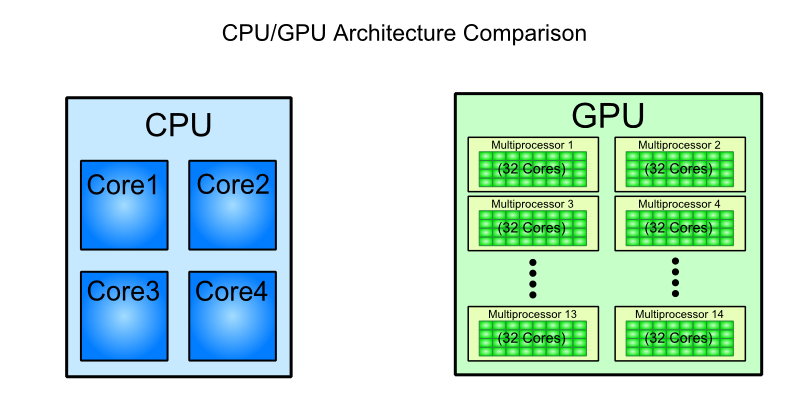
\includegraphics[scale = 0.5]{cpu_vs_gpu.png}
   \end{center}
  \caption{Différences entre un CPU et un GPU}
\end{figure}

\normalsize{

Contrairement au CPU qui possèdent un faible nombre de Cores, l’architecture des cartes GPU compte un ensemble de multiprocesseurs (ou SM pour Streaming Multiprocessor). Chacun de ces SM possèdent des unités de calculs, nommée Streaming Processor (SP). Un warp scheduler va permettre à un groupement de 32 SP nommés warps d'accéder à la mémoire.\\

Un thread GPU n’a pas tout à fait le même sens qu’un thread CPU. À l’inverse des threads CPU, les threads GPU sont extrêmement légers ce qui signifie qu’un changement de contexte est une opération peu coûteuse. Les nouvelles cartes NVDIA possèdent maintenant deux warp scheduler, contrairement aux anciens modèles qui n'en possédaient qu'un. Cela permet donc d'accélérer l'accès à la mémoire. \\
}

\begin{figure}[h]
   \begin{center}
   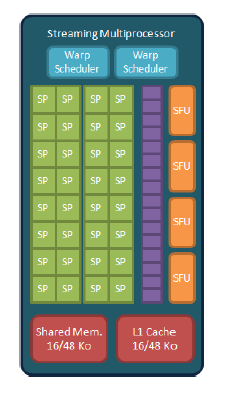
\includegraphics[scale = 0.8]{SM.png}
   \end{center}
  \caption{Architecture simplifiée d'un Streaming MultiProcessor d'une carte NVIDIA Fermi C2050, selon \cite{Passerat-Palmbach.etal.2011}}
\end{figure}


\section{Méthode de parallélisation}
\vspace{6mm}
\normalsize{
Afin de réaliser plusieurs réplications d'une simulation, permettant ainsi de réaliser un intervalle de confiance pour celle-ci, la parallélisation est utilisée depuis les années 90 sous le nom de MRIP (Multiple Replications in Parallel) \cite{Pawlikowski.etal.1994}. Chaque réplication est réalisée en parallèle.\\ \\

Depuis peu, on utilise des cartes graphiques afin de profiter de leur grand nombre de threads disponibles. Mais une des limites des GPU est la médiocrité de l'accès mémoire. En attendant une amélioration de la part des constructeurs, notamment par l'amélioration de la mémoire du GPU (GDDR), il est possible d'améliorer les performances grâce à une autre vision de la parallélisation du programme.\\ \\

\subsection{Le paradigme SIMT et le Thread Level Parallelism}
\vspace{6mm}
La méthode actuelle de parallélisation utilisée par OpenCl ou CUDA est le paradigme SIMT (Single Instruction Multiple Threads). C'est une amélioration du paradigme SIMD (Single Instruction, Multiple Data). Avec SMID, la même instruction est exécuté en parallèle avec des données différentes en entrées. \\


SIMT permet donc de réaliser plus facilement des applications GPU. Le développeur crée donc une seule fonction, appelée Kernel, et manipule les threads plutôt que les vecteurs utilisés en SIMD. \\

Ces kernels se subdivisent en blocs composés de warps . Un warp est un groupe de threads pour le scheduling, mais ce n'est pas une partie de circuit exécutant du code à part entière. Les kernels vont ensuite être exécutés sur un Streaming MultiProcessor. Chaque SM dispose d’une mémoire partagée ou Shared Memory. 

\subsection{Introduction au paradigme Warp-Level}
\vspace{6mm}
\normalsize{
Il existe toutefois deux problèmes pour l'application de ce paradigme à la réplication de simulations. En utilisant une réplication par thread, peu de threads sont utilisés. Hors, les performances des GPU sont optimales lorsque les cartes sont pleinement utilisées. Mais le principal problème est que, lorsque l'on réalise une simulation stochastique, les tirages de nombres aléatoires vont se faire au même point. Il va donc y avoir un problème pour les Threads appartenant à un même Warp. L'exécution se fera chacun son tour pour avoir accès à la mémoire, et l'exécution sera donc sérialisée. \\ 

C'est pour cette raison que l'objectif de notre projet est donc d'implémenter un nouveau paradigme palliant ces problèmes: Warp-Level Parallelism.\\
}

\subsection{Le paradigme Warp-Level}
\vspace{6mm}

\normalsize{
Pour accélérer l'exécution de plusieurs réplications d'une simulation stochastique, un autre paradigme a été créé : le Warp-Level Parallelism (WLP). En effet, pour prendre en compte les contraintes décrites précédemment, on décide de n'exécuter qu'un Thread par Warp. Ainsi, le Warp-Scheduler n'aura à réaliser que l'accès à la mémoire pour une seule réplication. Il n'y a donc plus les problèmes d'accès au même point de plusieurs Thread lors du tirage des nombres aléatoires. Par ailleurs, aucune branche divergente n'apparaît, ce qui évite les portions de code exécutées en série. \\ \\

Enfin, baser le calcul au niveau des warps permet de créer des threads virtuels, puisque 32 threads seront créés par warp. Ainsi, on augmente l'occupation de la carte, améliorant de ce fait l'ordonnancement. On autorise donc un seul Thread par warp à s'exécuter sur les 32 possibles.
}
\begin{figure}[h]
   \begin{center}
   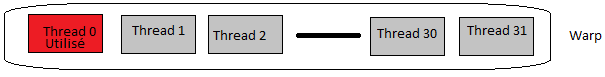
\includegraphics[scale = 0.9]{warp.png}
   \end{center}
  \caption{Exemple d'un Warp pour le Warp-Level Parallelisation}
  \label{warp_example}
\end{figure}

\newpage
 
\normalsize{
Sur la Figure \ref{warp_example}, on voit que seul le Thread 0 est activé dans son Warp. Les autres ne fonctionnent pas.\\

Après différents tests réalisés, on remarque pour une simulation simple avec un nombre de réplications situé entre 0 et 600 que les performances avec le paradigme Warp-Level Parallelism sont bien meilleures (ratio max x6) que pour le Thread Level Parallelism. Toutefois, arrivé à un très grand nombre de réplications ( $>$ 700 ), les performances convergent du fait du nombre limité de Warps pouvant être gérés par le GPU.\\
}

\normalsize{
La publication \cite{Passerat-Palmbach.etal.2011} ne fait état que d'une implémentation CUDA de ce paradigme. De plus, les auteurs soulignent l'intérêt d'une automatisation de la méthode, évitant à l'utilisateur d'insérer des lignes désactivant certains threads dans son code.
}

%%%%%%%%%%%%%%%%%%%%%%%%%%%%%%%%%%%%%%%%%%%%%%%%%%%%%%%%%%%%%%%%%%%%%%%%%%
% OpenCL

\chapter {OpenCL}

\section{Définition}
\vspace{6mm}
\normalsize{
OpenCL (Open Computing Langage) est un projet ambitieux, initialement lancé par Apple. Les spécifications ont été proposées et acceptées par le consortium Khronos, qui par ailleurs s'occupe aussi d'OpenGL.La première version officielle (1.0) est sortie en juin 2008. Actuellement, la version 1.2 de l'API est proposé aux fabriquant. Le but de ce projet est de permettre aux développeurs de tirer parti des énormes capacités de calcul des processeurs graphiques (GPUs) ou des processeurs classiques (CPUs) d'aujourd'hui. Chaque fabricant propose son implémentation de l'API pour le matériel qu'ils fournissent. Cette situation est ambiguë, car il existe une hétérogénéité dans leurs performances. Le cas de NVIDIA est symptomatique. En effet, NVIDIA est propriétaire de la plateforme CUDA qui est un concurrent direct d'OpenCL. Ce qui a été un frein pour le déploiement de l'API car NVIDIA possède 32\% de part de marché, et est leader dans le domaine des cartes graphiques haut de gamme.
}

\section{L'architecture}

\normalsize{
Voici un schéma representant l'architecture d'OpenCL.
}

\begin{figure}[h]
   \begin{center}
   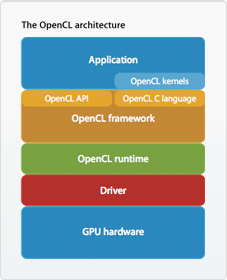
\includegraphics[scale = 0.60]{opencl_archi.png}
   \end{center}
  \caption{Architecture d'OpenCL.}
\end{figure}


\normalsize{
L'utilisation d'OpenCL peut se décomposer en deux partie. La première est la partie qui va manager le code à exécuter et la deuxième la partie du code qui va être directement exécuté sur la plateforme utilisée. Pour manager son code source OpenCL, l'API propose plusieurs étapes.\\
}

\begin{itemize}
\item Création d'un contexte selon le device que l'on veut utiliser (CPU ou GPU).
\item Allocation des buffers mémoire pour les entrées-sorties.
\item Récupération du code source à exécuter.
\item Création des kernels à exécuter.
\item Paramètrage du nombre d'e réplications à effectuer
\item Planification de l'exécution sur le device.\\
\end{itemize}

\normalsize{
Il est intéressant de noter que le code source des kernels peut être récupéré de plusieurs façons. Le kernel qui est dans l'exemple ci-dessous provient d'un fichier source que le programme va compiler directement à l'exécution. On peut aussi utiliser directement le binaire de la fonction ce qui permet d'éviter une phase de compilation qui peut être longue. Voici un exemple de code de création et de lancement de kernel. 
}

\begin{figure}[h]
   \begin{center}
   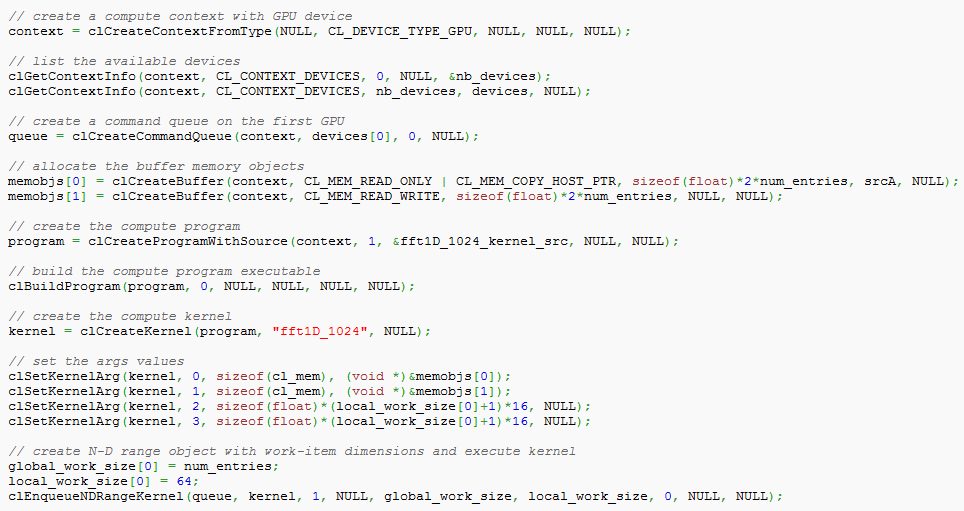
\includegraphics[scale = 0.60]{kernelOpencl.png}
   \end{center}
  \caption{Exemple de code source OpenCL.}
\end{figure}

\normalsize{
Le code source de calcul possède quelques particularités par rapport à un code classique en C. Un kernel est en effet toujours une fonction dont le prototype commence par le mot-clé {\bf \_\_kernel}. Pour la suite, on peut utiliser des fonctions permettant de récupérer des informations sur l'exécution du code à proprement parlé comme par exemple le numéro de work-item. Voici un exemple de code source pouvant être directement exécuté sur un device compatible OpenCL. 
}

\clearpage

\begin{figure}[h]
   \begin{center}
   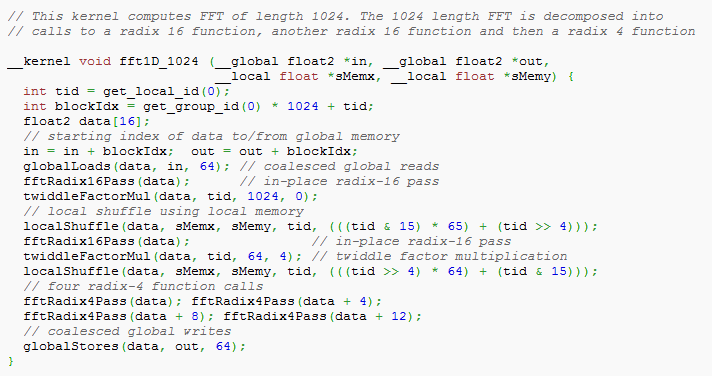
\includegraphics[scale = 0.78]{kernelOpenclCode.png}
   \end{center}
  \caption{Exemple de kernel OpenCL.}
\end{figure}

\normalsize{La décomposition de la partie calcul et de la partie scheduler est une fonctionnalité très interrésante. Car cela oblige aux développeurs à rendre leurs programmes plus modulaire. De plus, il est très facile pour une entité de créer un "launcher" universel qui permettra d'économiser du temps de dévellopement de la partie non-métier du programme.\\
}

\normalsize{
Pour conclure sur cette partie, on peut dire que OpenCL est une API qui a de l'avenir. En effet malgré certaines réticence de NVIDIA, OpenCL a été adopté par les autres constructeurs comme AMD ou Intel qui en font leur fer de lance. Intel propose désormais une implémentation matérielle d'OpenCL dans leurs derniers processeur basé sur l'architecture Ivy Bridge.
} 


\chapter{Les spécificités du Scala}

\section{Introduction}
\vspace{6mm}
\normalsize{
Scala est un langage de programmation multi-paradigme conçu à l'École polytechnique fédérale de Lausanne (EPFL) \cite{Odersky.etal.2004} pour exprimer les modèles de programmation courants dans une forme concise et élégante. Son nom vient de l'anglais Scalable language qui signifie à peu près « langage adaptable » ou « langage qui peut être mis à l'échelle ». Il peut en effet être vu comme un métalangage.\footnote{Langage qui permet la définition formelle d'un langage de programmation }\\
Ce chapitre montre les fonctionnalités avancées de ce langage qui ont été utilisées lors de ce projet.
}

\section{Object}
\vspace{6mm}
\normalsize{
Object est une particularité Scala. On peut s'en servir principalement de 3 façons, en singleton, en factory et pour finir en objet compagnons.
} 

\subsection{Singleton}
\vspace{6mm}
\normalsize{
Object est une particularité Scala. Cela permet d'implémenter très facilement le design patern {\bf singleton}. Pour l'utiliser, il suffit de remplacer le mot clé class par {\bf object} lors de la déclaration. {\bf object} n'est pas un élément qui peut être instancié. Donc il est impossible d'avoir plusieurs réplications de cet objet. On retrouve le comportement du design pattern Singleton. 
}

\begin{lstlisting}
object MaitreDuJeu () {
   def kick(...) = {...}
   def slay(...) = {...}
}
\end{lstlisting}

\normalsize{
\noindent
A l'appel, on obtiendra.
}

\begin{lstlisting}
MaitreDuJeu.kick(...)
MaitreDuJeu.slay(...)
\end{lstlisting}

\subsection{Factory}
\vspace{6mm}
\normalsize{
Une autre utilisation du type object est l'implémentation du design pattern factory. Il suffit de créer une méthode qui retourne l'objet créé. En voici un exemple ci-dessous.
}

\begin{lstlisting}
object JoueurFactory () {
   def creerJoueur(nom : String) : Joueur = {
      return new Joueur(nom);
   }
}
\end{lstlisting}

\subsection{Objet compagnon}
\vspace{6mm}
\normalsize{
La troisième et dernière utilisation présentée est la possibilité de l'associer à une classe de même nom et qui permettra à cette classe de posséder des attributs et des membres statiques. Voici une comparaison entre un code Scala et son équivalent Java.\\ \\
}

\begin{lstlisting}
class maClass {
    private int monAttr1;
    public static int monAttr2;

    public static void maMethode() {
       ...
    }
}
\end{lstlisting}
\vspace{6mm}
\begin{lstlisting}
class maClass() {
    private var monAttr1 : int ;

    object maClass {
       private var monAttr2 : int ;
       def maMethode() = {
          ...
    }
}
\end{lstlisting}

\section{Trait}

\normalsize{
Un trait est une classe abstraite, mais avec quelques particularités :
}

\begin{itemize}
\item Un trait est déclaré avec le mot clé "trait" alors que les classes abstraites le sont avec "abstract class".
\item On ne peut pas déclarer de champs dans le constructeur d'un trait, c'est à dire écrire val ou var avant le nom d'un argument du constructeur principal( cette restriction sera supprimée dans les prochaines versions de Scala). 
\item On peut hériter de plusieurs traits. \\
\end{itemize}

\newpage
\normalsize{
\noindent
Exemple :
}

\begin{lstlisting}
trait monTrait {
       def maMethode() = {...}
}
\end{lstlisting}
\vspace{6mm}


\normalsize{
Ce type de données est préféré aux classes abstraites car l'héritage, en Scala, possède un facteur bloquant. En effet, il est impossible pour une classe d'hériter de plusieurs classes abstraites. 
}

\section{La programmation fonctionnelle}
\vspace{6mm}
\normalsize{
La programmation fonctionnelle est un paradigme de programmation qui limite les effets de bords en interdisant les opérations d'affectation. Les programmes fonctionnels purs sont un ensemble de fonctions imbriquées les unes dans les autres. La contrainte principale de la programmation fonctionnelle est qu'une fonction ne peut avoir qu'une seule sortie.\\

 Il existe des langages, comme le Scala, qui peuvent utiliser à la fois le paradigme fonctionnel et le paradigme impératif. On appelle ces langages des langages impurs. Ils ont le gros avantage de pouvoir s'adapter au type de problèmes à résoudre au dépend de la baisse de robustesse engendrée par l'interdiction des opérations d'affectation.

\subsection{Les fonctions littérales}
\vspace{6mm}
\normalsize{
Concrètement, une fonction littérale est une fonction sans nom. Elle est souvent utilisée comme argument de fonction. Par exemple, la méthode foreach de la classe Array[T] prend une fonction en paramètre et va l'appliquer à tous les éléments contenus dans le tableau. Une fonction littérale se présente sous la forme suivante : \\
}

\begin{lstlisting}
(x:Int, y:Int) => x + y
\end{lstlisting}

\normalsize{
\noindent
où les arguments sont situés entre parenthèses, et le corps de la fonction est situé après la flèche.
}

\subsection{Le type fonction}
\vspace{6mm}
\normalsize{
L'une des faiblesses de Java est l'absence de pointeur de fonction. En effet, on ne peut pas passer une fonction en paramètre dans Java. Scala propose de corriger cela à l'aide du type fonction. Le Scala étant un langage tout objet, une fonction est un objet comme un autre. Elle  peut être affectée à une variable {\bf val} ou {\bf var}. Une variable fonction se déclare comme ceci:\\
}

\begin{lstlisting}
val sum : (int, int) : int =  (a : int, b : int) => a + b
val res = sum(4,5)
// res = 9
\end{lstlisting}
\newpage
\normalsize{
On remarque que pour la déclaration de sum, on définit le type {\bf int, int) : int}. Le prototype de la fonction donne le type de la variable. On peut utiliser le type fonction en paramètre de méthode. \\

Un exemple classique est l'implémentation d'une fonction qui applique un traitement spécifique à un objet passé en paramètre.\\
}

\begin{lstlisting}
def operation( x : int, y : int, op : (int,int) => int ) : int = { 
   op(x,y) 
}
\end{lstlisting}
\vspace{6mm}
\normalsize{
La méthode opération peut être appelée avec {\bf sum} comme paramètre, car il y a concordance entre leur prototype. On peut l'utiliser avec le code suivant.\\
}

 \begin{lstlisting}
val result = operation(2,3,sum)
// val = 5 
\end{lstlisting}
\vspace{6mm}

\normalsize{

	On retrouve ici le comportement des pointeurs de fonction en C, fonctionnalité que l'on peut simuler en Java, à l'aide d'une interface avec la méthode de calcul a implémenter. Une autre application est de faire des prédicats, utilisables sur des collections, à l'instar de la bibliothèque standard C++ (STL) sur la méthode {\bf sort}.\\
} 

\subsection{Les closures}
\vspace{6mm}
\normalsize{
Par définition, une closure est une fonction qui possède un état interne. C'est à dire que ce type de code s'exécute selon un contexte prédéfini avant. Cependant, la closure est toujours à l'écoute des variables qu'on lui a intégrées. L'exemple suivant va montrer plus en détail son fonctionnement classique.\\
}

 \begin{lstlisting}
def compteur( debut : int) = (x : int) => x + debut
val cpt1 = compteur(1);
// cpt1 est un pointeur de fonction
val res = cpt1(3);
// res = 4
\end{lstlisting}
\vspace{6mm}

\normalsize{
\noindent
L'exemple suivant montre quant à lui les effets externes après la déclaration de la closure.\\
}

 \begin{lstlisting}
var debut = 0;
def compteur = (x : int) => x + debut
val cpt1 = compteur();
// cpt1 est un pointeur de fonction
val res = cpt1(3);
// res = 3
debut = 10; // Modification de la variable initiale
val resModif = cpt1(5)
// resModif = 15
\end{lstlisting}

\normalsize{
On remarque que la modification de la variable {\bf debut} affecte le comportement de la closure. En effet, toutes les variables externes utilisées dans les closures sont des références. Donc  les valeurs prises en comptes sont les valeurs actuelles lors de l'appel de la fonction. 
}

\section{L'écriture de plugins de compilation}

\subsection{le compilateur Scala}
\normalsize{
Par définition, le compilateur scala se veut simple et flexible. La flexibilité provient du fait que l'on peut très facilement modifier le comportement du compilateur à l'aide de plugins externes. Attention, cette fonctionnalité doit être utilisé avec précaution. La norme Scala conseille de vérifier si des bibliothèque peuvent permettre d'implémenter le problème en questions. Il est recommandé d'utiliser des plugins dans les cas suivants :
} 
\begin{itemize}
\item Contrainte supplémentaire à la compilation ( Ajout de robustesse au code).
\item Optimisations à la compilation.
\item Modification de la syntaxe Scala.
\end{itemize}
\vspace{6mm}
\normalsize{

	L'avantage de l'utilisation de plugin est la non-modification du compilateur de base. En effet, les plugins disponibles sont distribuables de la même façon qu'une library. Un plugin peut être classé en deux catégories. La première est l'ajout d'une phase de compilation comme un pre-check ou transformation d'une partie de code spécifique. La deuxième est la modification du comportement des annotations. 
}

\subsection{Ajouter un plugin scala}
\normalsize{
Le plugin en exemple ci-dessous, propose de détecter les divisions par zéro évidente. Le code est tiré du cite officiel (www.scala-lang.org).
}

\begin{lstlisting}
class DivByZero(val global: Global) extends Plugin {
  import global._
  val name = "divbyzero"
  val description = "checks for division by zero"
  val components = List[PluginComponent](Component)
  
  private object Component extends PluginComponent {
    val global: DivByZero.this.global.type = DivByZero.this.global
    val runsAfter = "refchecks"
    val phaseName = DivByZero.this.name
    def newPhase(_prev: Phase) = new DivByZeroPhase(_prev)    
    
    class DivByZeroPhase(prev: Phase) extends StdPhase(prev) {
      override def name = DivByZero.this.name
      def apply(unit: CompilationUnit) {
        for ( tree @ Apply(Select(rcvr, nme.DIV), List())) <- unit.body;
             if rcvr.tpe <:< definitions.IntClass.tpe) {
            unit.error(tree.pos, "definitely division by zero")
          }
      }
    }
  }
}
\end{lstlisting}

\normalsize{
Le code du plugin est composé d'une seule classe dérivante de Plugin. Elle possède un seul paramètre pour son constructeur qui est de type {\bf global}. Le plugin doit définir au minimum un object dérivant PluginComponent.\\

 Le nom des object doivent être inclus dans la liste {\bf components}. De plus, chaque composant doit définir une méthode {\bf newPhase} qui crée la phase du compilateur. Et pour finir, chaque phase doit redéfinir la méthode {\bf apply} pour implémenter la partie concrète du compilateur.\\
}

\normalsize{
Comme on peut l'apercevoir au travers de l'exemple précédent, la réalisation d'un plugin Scala est une tâche extrêmement légère par rapport à la modification d'un compilateur libre d'un langage comme le C. Cette fonctionnalité a un fort potentiel pour la création d'environnement de développement robuste et fiable. On pourrait penser que dans l'avenir, ce genre de mécanisme permettra au Scala d'être facilement maintenable par des communautés de développeurs.
}

\chapter{ScalaCL}

\section{Introduction}
\vspace{6mm}
\normalsize{
ScalaCL est un langage dédié \footnote{ Langage de programmation dont les spécifications sont dédiées à un domaine d'application précis} développé par Olivier Chafik. ScalaCL est scindé en deux parties. La première est ScalaCLCollections qui réécris les collections standards de Scala, en l'adaptant au contexte OpenCL.\\

 La deuxième et dernière partie est un plugin de compilation Scala permettant d'utiliser les éléments implémentés dans ScalaCLCollections. L'objectif final est d'obtenir un programme exécutable sur un GP-GPU en utilisant l'API OpenCL. Depuis peu, ScalaCL a été intégré au projet nativelibs4java \footnote{Repository de library d'inter-opérabilité entre Java/Scala et C, C++, ObjectiveC}.
}

\section{Description de l'architecture}

\subsection{ScalaCLCollections}
\vspace{6mm}
\normalsize{
D'un point de vue modélisation, ScalaCLCollections est composé de deux parties. La première est la réécriture de collections Scala et la seconde est une modélisation de méthodes appelées avec OpenCL. Actuellement, trois collections ont été implémentées.
}

\begin{itemize}
\item CLArray[T].
\item CLFilteredArray[T].
\item CLFunction[A,B].\\
\end{itemize}

\normalsize{
CLArray et CLFiltered reprennent le comportement des classes issues des collections standards de Scala. Cependant, des fonctionnalités ont été ajoutées. Elles possèdent une structure asynchrone. En effet, il est impossible de lire une donnée en cours de lecture et vice-versa. Ce comportement est quasi-indispensable dans des environnements hautement parallèles.\\

CLFunction se situe entre le modèle et les collections car le plugin ScalaCL convertit les fonctions écrites en Scala en instance de CLFunction. Cependant, il est possible de créer manuellement cette instance afin de travailler au plus près des collections.  Cette méthode est tout de même déconseillé car le plugin permet d'optimiser la fonction modéliser.}

\normalsize{
 Voici un exemple de code utilisant directement CLFunction:
}
\begin{lstlisting}
def testMapArrayCapture {
    val rg = (0 until n).map(_ * 10).toCLArray

    val f: CLFunction[Int, Int] =
      (
        (x: Int) => rg(x) - x, 
        Array("_1[_] - _"),
        impl.CapturedIOs(
          Array(IntCLDataIO.asInstanceOf[CLDataIO[Any]]),
          Array(),
          Array()
        )
      )


    val fCapt = f.withCapture(
      Array(rg.asInstanceOf[CLArray[Any]]),
      Array(),
      Array()
    )
    same(a.map(fCapt), cla.map(fCapt))
  }
\end{lstlisting}

\vspace{6mm}

\normalsize{
La modélisation comporte plusieurs caractères intéressants.  En effet, il s'agit d'un modèle très complet qui gère toutes les fonctionnalités et les particularités des fonctions. Voici un diagramme UML simplifié pour voir comment sont articulés ces éléments.
}

\begin{figure}[h]
   \begin{center}
   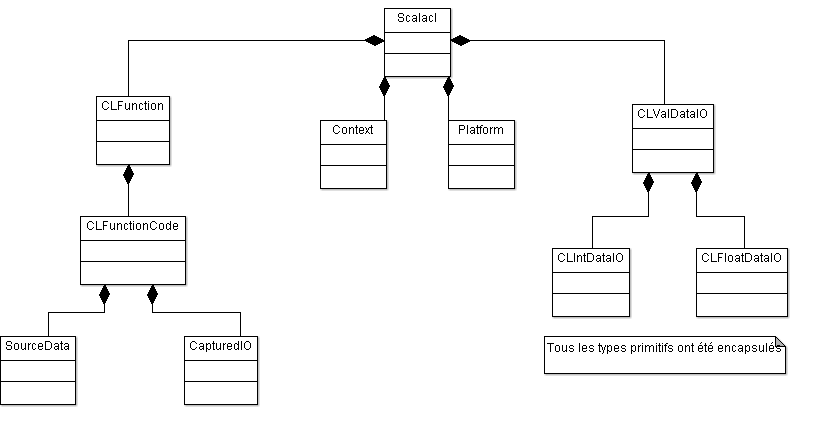
\includegraphics[scale = 0.60]{ClassScalaClcollection.png}
   \end{center}
  \caption{Diagramme UML simplifié de ScalaCLCollections.}
\end{figure}
\newpage
\normalsize{
On remarque que ce diagramme peut être décomposé en trois parties distinctes. La première regroupe {\bf CLFunction} et ses classes filles. Elles servent à modéliser les fonctions en terme d'exécution. {\bf SourceData} comporte la partie métier du code tandis que {\bf CapturedIO} se concentre sur la gestion de la mémoire pour les paramètres d'entrée et la/les valeur(s) de sortie.\\
}

\normalsize{
La deuxième, {CLValDataIO} et ses classes filles permettent l'encapsulation des types primitifs issus d'OpenCL. Les types implémentés sont :
}

\begin{itemize}
\item Booléen.
\item Byte.
\item Char.
\item Double.
\item Float.
\item Int.
\item Long.
\item Short.
\item Tuple. \\
\end{itemize}

\normalsize{
La troisième et dernière partie assemble {\bf Scalacl}, {\bf Context}, {\bf Platform}. Ces trois classes contiennent des informations sur les conditions d'exécution de la fonction. {\bf Platform} s'occupe de la partie hardware de la machine où est exécuté le code. Tandis que {\bf Context} se concentre sur le device utilisé (CPU ou GPU). 
}

\subsection{ScalaCLPlugin}
\vspace{6mm}
\normalsize{
La fonction principale du plugin est d'analyser le code Scala utilisant ScalaCLCollection pour le tranformer en CLFunction puis en code C/C++ OpenCL. L'architecture de la partie plugin est vraiment très intéressante. En effet, Olivier Chaffik l'a développé de manière à être très modulaire et robuste. Elle est constituée d'un noyau qui implémente une interface pour chaque fonctionnalité. Voici un diagramme UML qui résume l'architecture.
}

\begin{figure}[h]
   \begin{center}
   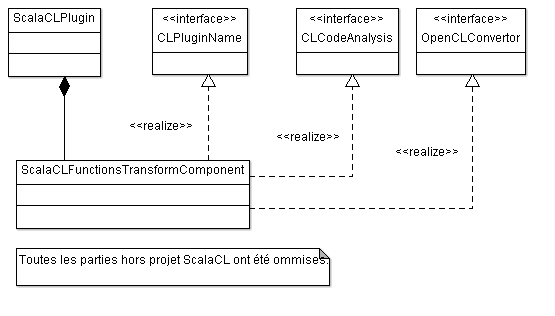
\includegraphics[scale = 0.65]{ClassScalaClPlugin.png}
   \end{center}
  \caption{Diagramme UML simplifié de ScalaCLPlugin.}
\end{figure}

\normalsize{
La fonction noyau décrite dans le paragraphe précédent est {\bf ScalaCLFunctionTransformComponant}. Elle contient tout la partie fixe du code du plugin. Son objectif principal est d'analyser le code et de le transformer en modèle CLFunction. Cette classe implémente plusieurs interfaces.\\

 {\bf CLPluginName} définit les éléments comme le package de collections qui seront utilisés pour la construction de la CLFunction. {\bf CLCodeAnalysis} donne, quant à lui, des compléments sur la lecture et la transformation du code Scala lu.\\

 {\bf OpenCLConverter} est le trait qui transforme le modèle CLFunction en langage C/C++. Cette partie du code est très critique. La moindre modification peut entrainer des erreurs difficiles à résoudre. C'est pour cela qu'il est déconseillé de modifier cette implémentation de ce trait.\\
} 

\section{Insertion du WLP dans ScalaCL}
\vspace{6mm}
\subsection{Introduction}
\vspace{6mm}
\normalsize{
L'objectif final de ce projet était d'insérer le paradigme Warp-Level dans le projet ScalaCL. Après plusieurs échanges avec Olivier Chafik, nous avons conclu sur la démarche à réaliser pour implémenter cette nouvelle fonctionnalité. Les modifications ont été faite sur les deux composantes du projet, la partie Collection et la partie Plugin.\\
}

\subsection{Modifications sur ScalaCLCollection}
\vspace{6mm}
\normalsize{
Pour commencer, il a fallu modifier le modèle de CLFunctionCode. En effet, l'implémentation du paradigme Warp-Level nécessitant d'effectuer un test au début du code du kernel. C'est pour cela que deux paramètres ont été ajouté à la méthode {\bf buildSourceData} de CLFunctionCode. il s'agit de {\bf bodyPrefix} et de {\bf bodySuffix}. Ces deux paramètres sont des éléments qui seront insérés systématiquement en début et en fin du kernel. Voici une partie du code utilisant cette fonctionnalité.
}

\begin{lstlisting}
outputFunction(
      "__kernel void array_array",
      Seq(sizeParam, kernelParams),
      Seq(
        bodyPrefix,
        indexHeader, 
        sizeHeader,
        kernDeclsArray,
        assigntArray,
        bodySuffix
      ),
      kernelsSource
    )
\end{lstlisting}

\normalsize{
Par ailleurs, Olivier Chafik, nous a conseillé de créer un nouveau package pour mieux exploiter la modification précédente. Le nouveau package obtenue est scalaclWLP. Il reprend la quasi-totalité du code du package scalacl. En effet, dans notre cas, il était pas nécessaire d'apporter des modifications aux collections. La modification se fera uniquement dans la déclaration de la méthode {\bf buildSourceData}.\\

Le test à ajouter pour le paradigme Warp-Level est constant. La solution retenue a été de modifier la valeur par défaut des paramètres {\bf bodyPrefix} et {\bf bodySuffix}. Voici la déclaration originale de la méthode buildSourceData.\\
}

\begin{lstlisting}
 def buildSourceData[A, B](
    outerDeclarations: Array[String],
    declarations: Array[String],
    expressions: Array[String],
    includedSources: Array[String],
    extraArgsIOs: CapturedIOs = CapturedIOs(),
    bodyPrefix: Array[String] = Array(),
    bodySuffix: Array[String] = Array()
  )
\end{lstlisting}
\vspace{6mm}
\normalsize{
\noindent
Voici la version adapté pour le paradigme Warp-Level.\\
}

\begin{lstlisting}
 def buildSourceData[A, B](
    outerDeclarations: Array[String],
    declarations: Array[String],
    expressions: Array[String],
    includedSources: Array[String],
    extraArgsIOs: CapturedIOs = CapturedIOs(),
    bodyPrefix: Array[String] = Array("if(get_global_id(0)==0){"),
    bodySuffix: Array[String] = Array("}")
  )
\end{lstlisting}
\vspace{6mm}
\normalsize{

Cette solution n'est sans doute pas la plus propre en terme de génie logiciel. Elle a cependant l'avantage de ne pas trop modifier l'architecture globale de ScalaCLCollection. L'autre solution aurait été de garder un seul package et d'implémenter une buildWLPSourceData qui aurait été appelé selon le paradigme que l'on veut utiliser.
}

\newpage
\subsection{Modifications sur ScalaCLPlugin}
\vspace{6mm}
\normalsize{
Comme l'avait conseillé Olivier Chafik nous avons créer un nouveau plugin pour ScalaCL. Tout comme avec la partie Collection du projet, il y a une grande majorité du code en commun.\\

Nous avons utilisé la même architecture que le plugin existant. C'est à dire un noyau ScalaFunctionsTransformComponant implémentant plusieurs interfaces. La majeure partie du travail a consister a connecter les modifications qui ont été faite sur les Collections. Pour cela, l'interface CLPlugin a été retouché pour obtenir {\bf CLWLPPluginName}. \\

Voici la nouvelle implémentation du trait
\vspace{6mm}
\vspace{6mm}
\begin{lstlisting}
  val ScalaCLPackage       = M("scalaclWLP")
  val ScalaCLPackageClass  = ScalaCLPackage.tpe.typeSymbol
  val CLDataIOClass = C("scalaclWLP.impl.CLDataIO")
  val CLArrayClass = C("scalaclWLP.CLArray")
  val CLFunctionClass = C("scalaclWLP.impl.CLFunction")
  val CLRangeClass = C("scalaclWLP.CLRange")
  val CLCollectionClass = C("scalaclWLP.CLCollection")
  val CLFilteredArrayClass = C("scalaclWLP.CLFilteredArray")
  val scalacl_ = N("scalacl")
  val getCachedFunctionName = N("getWLPCachedFunction")
  val Function2CLFunctionName = N("Function2CLFunction")
  val withCaptureName = N("withCapture")
\end{lstlisting}
\vspace{6mm}\vspace{6mm}
\normalsize{

Le paradigme Warp-Level ne nécessitant pas une analyse ou une écriture particulière du code. Il n'a pas été de corriger fondamentalement {\bf CLCodeAnalysis} et {\bf OpenCLConvertor} mis à part les liaisons avec CLWLPPluginName.\\
}

\normalsize{
Le noyau, quant à lui, a subi plusieurs transformations. La première est le choix des interfaces à implémenter. Au lieu de CLCodeAnalysis et CLPluginNames, on obtient CLWLPCodeAnalysis et CLWLPPluginNames.\\

C'est grâce à CLWLPPluginName que le plugin appellera désormais getWLPCachedFunction au lieu de getCachedFunction qui est situé dans ScalaCLCollections.
}

\newpage
\section{Premiers résultats}
\vspace{6mm}
\normalsize{
L'objectif de ce projet sera atteins si les kernels générés par ScalaCL comporteront le test initial en début de code. Pour vérifier ceci, nous avons utilisé la variable d'environnement               {\bf SCALACL\_VERBOSE} . Elle permet d'afficher une grande partie des traces d'executions de ScalaCL. Voici un code de test de notre implémentation.
}
\vspace{6mm}
\begin{lstlisting}
    def main(args: Array[String]) {

    implicit val context = Context.best(GPU)
    val filt = (
      (x: Int) => (x % 2) == 0, 
      Array("(_%2)==0")
    ): CLFunction[Int, Boolean]
    
    for (dim <- 1 until 1000) {
      val openclArray = (0 until dim).toCLArray.filter(filt).toArray.toSeq
      val openclRangePre: CLIndexedSeq[Int] = (0 until dim).cl.filter(filt)
      val openclRange = openclRangePre.toArray.toSeq
      val scala = (0 until dim).toArray.filter(filt).toArray.toSeq
      }
   }
\end{lstlisting}

\vspace{6mm}
\normalsize{
\noindent
On obtient donc en sortie :
}

\begin{figure}[h]
   \begin{center}
   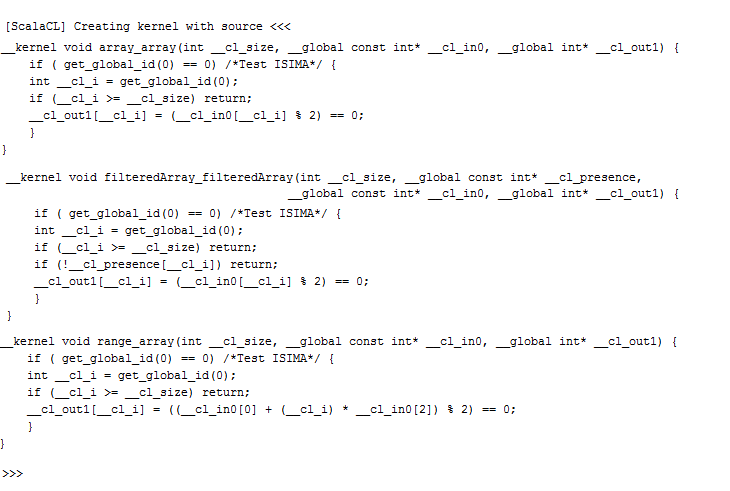
\includegraphics[scale = 0.9]{resultats.png}
   \end{center}
  \caption{Sortie en mode VERBOSE}
\end{figure}
\newpage
\normalsize{
On remarque que pour chaque kernel généré, on obtient bien le test inséré dans la méthode buildSourceData de CLFunction. Donc pour un code donnée, on peut obtenir sa version dans ce nouveau paradigme.
}




\newpage
\begin{flushleft}
\LARGE{ \bf {Conclusion}\bigskip}
\end{flushleft}
\vspace{10mm}
\normalsize
{

Lors de ce projet, nous avons réalisé une étude approfondie de l'ensemble des notions nous permettant de mener ce projet à terme. Nous avons d'abord analyser la publication sur laquelle le projet s'est basé. Nous avons donc étudié les différents paradigmes de programmation sur GP-GPU, afin de comprendre les subtilités et les avantages de l'utilisation du Warp-Level-Paradigm dans le cadre de la réplication d'expérience.\\ 

Nous avons ensuite étudié Scala, afin de comprendre les fonctionnalités et les particularités de ce langage. Ce langage novateur apporte une nouvelle dimension dans le monde de la programmation. En effet, il était assez difficile pour nous d'imaginer un langage qui puisse être autant adaptable aux besoins de l'utilisateur. Il ne fait aucun doute que le Scala sera bientôt un langage phare. \\

La plus grande partie du projet a ensuite été l'étude de l'architecture ScalaCL, afin de savoir comment on pourrait intégrer le paradigme Warp-Level sans modifier le comportement du code existant.
Cette partie a été notre plus grande difficulté. En effet, ScalaCL est un projet récent et ambitieux , et peu d'informations sont disponibles. Les nombreuses mises à jour, modifiant les parties. dans lesquelles nous avions insérer notre fonctionnalité nous a également posé problème.\\

Nous avons finalement réussi à implémenter le Warp-Level-Parallelism avec ScalaCL. Il est désormais possible de proposer nos modifications, afin qu'elles puissent être intégrer finalement dans la branche principale projet.
}

\begin{thebibliography}{10}
\providecommand{\url}[1]{#1}
\csname url@samestyle\endcsname
\providecommand{\newblock}{\relax}
\providecommand{\bibinfo}[2]{#2}
\providecommand{\BIBentrySTDinterwordspacing}{\spaceskip=0pt\relax}
\providecommand{\BIBentryALTinterwordstretchfactor}{4}
\providecommand{\BIBentryALTinterwordspacing}{\spaceskip=\fontdimen2\font plus
\BIBentryALTinterwordstretchfactor\fontdimen3\font minus
  \fontdimen4\font\relax}
\providecommand{\BIBforeignlanguage}[2]{{%
\expandafter\ifx\csname l@#1\endcsname\relax
\else
\language=\csname l@#1\endcsname
\fi
#2}}
\providecommand{\BIBdecl}{\relax}
\BIBdecl


\bibitem[PASSERAT 2011]{Passerat-Palmbach.etal.2011}
J.~{Passerat-Palmbach}, J.~Caux, P.~Siregar, and D.~Hill, ``Warp-level
  parallelism: Enabling multiple replications in parallel on gpu,'' in
  \emph{Proceedings of the European Simulation and Modeling Conference 2011},
  2011, pp. 76--83, iSBN: 978-90-77381-66-3.

\bibitem[PAWLIKOWSKI 1994]{Pawlikowski.etal.1994}
Pawlikowski, K., Yau, V., and McNickle, D. (1994).
Distributed stochastic discrete-event simulation in parallel time
  streams.
 In {\em Proceedings of the 26th conference on Winter simulation},
  pages 723--730. Society for Computer Simulation International.


\bibitem[ODERSKY]{Odersky.etal.2004}
M.~Odersky, P.~Altherr, V.~Cremet, B.~Emir, S.~Maneth, S.~Micheloud,
  N.~Mihaylov, M.~Schinz, E.~Stenman, and M.~Zenger, ``An overview of the scala
  programming language,'' Technical Report IC/2004/64, EPFL Lausanne,
  Switzerland, Tech. Rep., 2004.

\end{thebibliography}

%%%%%%%%%%%%%%%%%%%%%%%%%%%%%%%%%%%%%%%%%%%%%%%%%%%
\end{document}